\documentclass{article}

\usepackage{amsmath,amsfonts}
\usepackage[a4paper,margin=3cm]{geometry}
\usepackage{graphicx}

\setlength{\parindent}{0pt}

\title{IQB aufgaben}
\author{}
\date{}

\begin{document}
\maketitle

\section*{2021-4}
Gegeben sind die in $\mathbb{R}$ definierte Funktionen $f$ und $g$. Der Graph
von $f$ ist symmetrische bez\"uglich der y-Achse, Der Graph von $g$ ist
symmetrisch bez\"uglich des Koordinatenursprungs. Beide Graphhen haben einen
Hochpunkt im Punkt (2|1).

\begin{enumerate}
  \item[a)] Geben Sie f\"ur die Graphen von $f$ und $g$ jeweils die Koorinaten
    und die Art eines weiteren Extrempunkts an.

  \item[b)] Untersuchen Sie die in $\mathbb{R}$ definierte Funktion $h$ mit
    $h(x)=f(h)\cdot (g(x))^3$ im Hinblick auf einen m\"ogliche Symetrie ihres
    Graphen.

\end{enumerate}

\clearpage
\section*{2021-5}
\begin{minipage}{0.65\textwidth}
  Die Abbildung zeigt den Graphen $G_f$ einer in $\mathbb{R}$ definierten
  Funktion $f$ sowie den Graphen der ersten Ableitungsfunktion von $f$.

\begin{enumerate}
  \item[a)] Geben Sie die Steigung der Tangete an $G_f$ im Punkt $\left(0|f(0)\right)$ an.

  \item[b)] Betrachtet man die Schar der Funktionen $g_c$ mit $c\in
    \mathbb{R}^+$. Der Graph von $g_c$ geht aus $G_f$ durch die Streckung mit
    dem Faktor $c$ in y-Richtung hervor. Die Tangente an den Grphen von $g_c$
    im Punkt $(0|g_c(0))$ schneidet die x-Achse. Bestimmen Sie rechnerisch die
    x-Koordinate des Schnittpunkts.

\end{enumerate}

\end{minipage}
\hfill
\begin{minipage}{0.3\textwidth}
  \begin{center}
      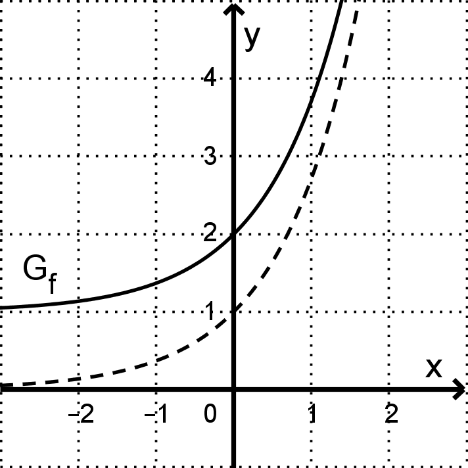
\includegraphics[width=\textwidth]{/home/daniel/documents/docs/LaTeX/misc/mathe-abi/i21-5.png}
  \end{center}
\end{minipage}

\clearpage

\section*{2022-2}
Gegeben sind die in $\mathbb{R}$ definierten ganzrationalen Funktionen
\[f_k:x \mapsto x^4 + (2-k) \cdot x^3 -k \cdot x^2 \text{ mit } k\in\mathbb{R}\]

\begin{enumerate}
  \item[a)] Begr\"unden Sie, dass der Graph von $f_2$ symmetrisch bez\"uglich der y-Achse ist.

  \item[b)] Es gibt einen Wert von $k$, f\"ur den 1 eine Wendestelle von $f_k$
    ist. Berechnen Sie diesen Wert von $k$.
\end{enumerate}

\vfill

\textit{Hilfe}

Die Schreibweise beschreibt eine Funktion $f_k$, die für jeden Wert von $k$
definiert ist. Die Funktion $f_k$ ist eine Funktion von $x$, dargestellt durch
die Zuordnung $x\mapsto x^4 + (2-k) \cdot x^3 -k \cdot x^2$. Das Symbol
$\mapsto$ bedeutet "wird abgebildet auf" und zeigt die Zuordnung von Werten in
der Domäne der Funktion (in diesem Fall reelle Zahlen) zu den entsprechenden
Funktionswerten in der Zielmenge (in diesem Fall ebenfalls reelle Zahlen).

Die Funktion $f_k$ hat auch eine Einschränkung: Der Parameter $k$ muss eine
reelle Zahl sein. Der Ausdruck "mit $k\in\mathbb{R}$" bedeutet, dass $k$ eine
beliebige reelle Zahl sein kann.

Die Funktion $f_k$ hat eine bestimmte algebraische Struktur, die durch die
Formel $x^4 + (2-k) \cdot x^3 -k \cdot x^2$ beschrieben wird. Der Parameter $k$
beeinflusst die Funktion, indem er die Koeffizienten der einzelnen Potenzen von
$x$ modifiziert. Wenn Sie den Wert von $k$ ändern, ändert sich auch das
Verhalten der Funktion.


\clearpage
\section*{2022-3}
Gegeben sind die in $\mathbb{R}$ definierten Funktionen 
\[f:x\mapsto \cos x \quad\text{und}\quad g_k:x\mapsto k\cdot x^2 \quad
\text{mit}\quad k\in\mathbb{R}^+.\]
Die Abbildung zeigt die Graphen von $f$ und $g_{\frac{1}{50}}$.

\begin{center}
    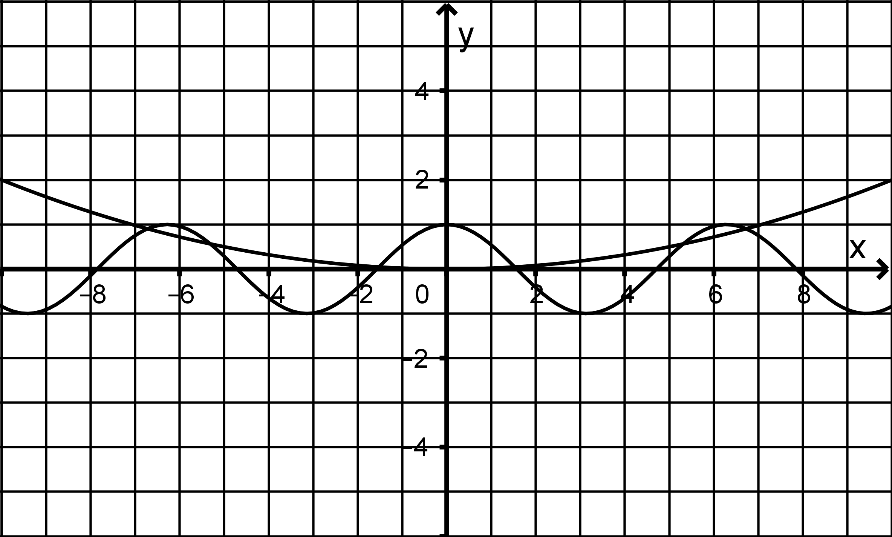
\includegraphics[width=.7\textwidth]{/home/daniel/documents/docs/LaTeX/misc/mathe-abi/i22-3.png}
\end{center}

\begin{enumerate}
  \item[a)] Skizzieren Sie in der Abbildung den Graphen von $g_{\frac{1}{4}}$.

  \item[b)] Entscheiden Sie, ob es Werte von k gibt, f\"ur die die Gleichung
    $f(x)=g_k(x)$ mehr als 2022 L\"osungen hat. Begr\"unden Sie ihre
    Entscheidung.
\end{enumerate}

\end{document}
